\chapter{Implementation of Bayesian Neural Fields}
\label{ch:bayesnf}

This chapter documents the third interpolation pipeline of the thesis,
the Bayesian Neural Field (BayesNF) of Saad et al.~\cite{saad2024bnf}
introduced in Section~\ref{sec:theory-bayesnf}. The implementation uses
the reference \texttt{google/bayesnf} library~\cite{bayesnfRepo} and
shares the data preparation, the spatial cross-validation partition and
the holdout reservation with the kriging and gradient-boosting
pipelines. The remaining design choices that are specific to BayesNF are
the architecture and posterior-inference hyperparameters, the temporal
seasonality encoding, the spatial covariate set, the interaction list
and the choice of inference scheme. Each of these is fixed by an
ablation reported in the following sections.

%=============================================================================
\section{Training data and target discretisation}
\label{sec:bayesnf-data}
%=============================================================================

The BayesNF model consumes the same long-table partition as the
LightGBM pipeline of Chapter~\ref{ch:gbm}: 1{,}966 training stations
split into five spatial folds (cf.\
Section~\ref{sec:kriging-cv-methodology}), 492 holdout stations
reserved for the cross-method evaluation of
Chapter~\ref{ch:comparison}, and the dynamic geo-feature set of
Section~\ref{sec:lgbm-features} recomputed per fold from the
training-fold neighbour pool. The single BayesNF-specific transformation
is the discretisation of the precipitation amount required by the
\texttt{NB} and \texttt{ZINB} likelihoods of
Section~\ref{sec:theory-bayesnf} (the chosen observation family is
\texttt{ZINB}, justified there). The continuous daily total in
millimetres is mapped to a non-negative integer at $0{.}1$~mm precision,
\begin{equation}
  y_{\mathrm{int}}(\mathbf{s},t) \;=\;
  \mathrm{round}\!\bigl(10\, y(\mathbf{s},t)\bigr)
    \;\in\; \mathbb{N}_{0},
  \label{eq:bnf-discretisation}
\end{equation}
and the inverse map $\hat{y}(\mathbf{s},t) = \hat{y}_{\mathrm{int}}/10$
is applied to the predictive mean and to every quantile after inference.
The factor of ten preserves the precision of the source records
(ReKIS rounds to $0{.}1$~mm) and is small enough that the
discretisation error is negligible against the standard deviation of
the daily precipitation. No additional preprocessing of the target is
required.

%=============================================================================
\section{Architecture and posterior hyperparameters}
\label{sec:bayesnf-arch}
%=============================================================================

The architecture follows the defaults recommended by Saad et al.\
\cite{saad2024bnf} and the reference repository~\cite{bayesnfRepo}: two
hidden layers of width $256$, the mixed-activation block of
Section~\ref{sec:theory-bayesnf-arch}, and the spatial Fourier feature
encoding of Equation~\eqref{eq:bnf-spatial-fourier}. The covariate scaling
layer is enabled and absorbs the per-feature standardisation, so all
non-temporal inputs are fed unmodified to the network. The
\texttt{ZINB} observation layer has one global zero-inflation
probability $\pi_0$ and one global negative-binomial dispersion shape
$\alpha$, both learned jointly with the network weights.

\paragraph{Ensemble size.} The mean-field posterior is non-convex and
the optimiser converges to a different mode for each random seed; the
standard remedy is to fit several VI replicas with independent
initialisations and average their predictive distributions. Saad et
al.\ report runtime-versus-error profiles of VI, MAP and MLE on a set
of spatiotemporal benchmarks (Fig.~6 of~\cite{saad2024bnf}) in which
the predictive error of the variational scheme flattens between
sixteen and thirty-two replicas; the same value
$\texttt{ensemble\_size} = 32$ is adopted here.

\paragraph{Number of epochs.} The training horizon
$\texttt{num\_epochs} = 100$ is set empirically:
Figure~\ref{fig:bnf-kfold-losses} shows the per-step ELBO of the five
k-fold VI runs, which collapse to a tight band well before epoch $100$
and stay on a shallow plateau thereafter.

\begin{figure}[ht]
  \centering
  \includegraphics[width=\linewidth]{images/06/bnf_kfold_losses.pdf}
  \caption{Per-step ELBO loss of the five spatial k-fold VI runs across
  the $100$-epoch schedule. Left: linear axis. Right: log axis. Each
  fold is drawn as a faint envelope of its $32$ VI members plus the
  per-fold ensemble mean (solid line)}
  \label{fig:bnf-kfold-losses}
\end{figure}

%=============================================================================
\section{Temporal seasonality ablation}
\label{sec:bayesnf-seasonality}
%=============================================================================

Two periods are plausible candidates for daily precipitation in central
Europe: the annual cycle $p = 365{.}25$~d, which carries the dominant
winter--summer modulation of frontal systems, and the weekly cycle
$p = 7$~d, sometimes detectable as a low-amplitude fingerprint of
synoptic regimes. The maximum harmonic count tested, $H = 10$, resolves
features as short as $\approx 18$~d within the annual cycle.

To attribute any difference between two seasonality configurations to
seasonality alone rather than to a different baseline of spatial
information, the ablation is run on a deliberately minimal feature set:
time, the two raw coordinates $(\text{lat}, \text{lon})$, the static
\texttt{elevation\_m}, and the six SoilGrids covariates of
Section~\ref{sec:precip_statistics}; none of the neighbour-derived
geo-features of Section~\ref{sec:lgbm-features} is included. Six configurations are
evaluated on fold~0 of the canonical five-fold partition, restricted
to the five-year window 2018--2022 and with $\texttt{ensemble\_size} =
4$ to keep the ablation budget within a single GPU-day; all other
hyperparameters match Table~\ref{tab:bnf-hyperparams}.

\begin{table}[ht]
  \centering
  \caption[Seasonality ablation on fold~0]{Seasonality ablation. CRPS,
  MAE and RMSE on the held-out stations of fold~0 (5-year window, no
  geo-features, $\texttt{ensemble\_size}=4$). Lower is better for every
  metric. The configuration adopted for all subsequent experiments is
  in bold}
  \label{tab:bnf-seasonality}
  \begin{tabular}{l c c c c c}
    \toprule
    Configuration         & $|P|$ & $H_p$
                          & CRPS  & CRPS$_{\mathrm{wet}}$
                          & RMSE                            \\
    \midrule
    \texttt{Y\_h1}        & 1 & $[1]$
                          & 1.659 & 3.074 & 3.929           \\
    \texttt{Y\_h3}        & 1 & $[3]$
                          & 1.505 & 3.087 & 3.368           \\
    \texttt{Y\_h4}        & 1 & $[4]$
                          & 1.534 & 3.165 & 3.413           \\
    \texttt{Y\_h10}       & 1 & $[10]$
                          & 1.347 & 3.110 & 2.603           \\
    \texttt{WY\_h1\_4}    & 2 & $[1, 4]$
                          & 1.324 & 3.235 & 2.427           \\
    \textbf{\texttt{WY\_h1\_10}} & 2 & $[1, 10]$
                          & \textbf{1.067} & \textbf{2.688} & \textbf{2.012} \\
    \bottomrule
  \end{tabular}
\end{table}

The ranking in Table~\ref{tab:bnf-seasonality} is monotone in the
expected direction. Within the annual-only family, increasing the
harmonic count from one to ten reduces CRPS from $1.659$ to $1.347$,
a relative improvement of approximately $19\%$, which confirms that
the within-year structure of central-European precipitation is too
sharp to be captured by a single sinusoid. Adding a one-harmonic
weekly cycle on top of the four annual harmonics
(\texttt{WY\_h1\_4}) gives a small additional improvement over
\texttt{Y\_h4} but is dominated by the deeper annual encoding of
\texttt{Y\_h10}. The combination \texttt{WY\_h1\_10}, which carries
both a weekly cycle and the ten-harmonic annual encoding, attains
$\mathrm{CRPS} = 1.067$, an improvement of approximately $21\%$ over
the best annual-only configuration \texttt{Y\_h10}, and is the global
minimum on every metric in the table including the wet-only CRPS.
This configuration is fixed for all subsequent experiments and is
recorded as such in Table~\ref{tab:bnf-hyperparams}.

%=============================================================================
\section{Spatial covariates and neighbour-derived features}
\label{sec:bayesnf-features}
%=============================================================================

Once the seasonality is fixed, the second set of design choices
concerns the spatial side of the input vector. BayesNF places the
spatial Fourier features of Equation~\eqref{eq:bnf-spatial-fourier} on
the raw $(\text{lat}, \text{lon})$ inputs, so the network already has a
rich self-built spatial representation; any additional covariate must
add information that is not derivable from coordinates alone. The
covariates considered here are the same dynamic geo-features used by
the LightGBM pipeline (Section~\ref{sec:lgbm-features}), the
\texttt{elevation\_m} from the Copernicus DEM, and the six SoilGrids
predictors (Section~\ref{sec:precip_statistics}).

The full feature inventory consumed by BayesNF is listed in
Table~\ref{tab:bnf-features}. It comprises the time index, the two raw
coordinates, the elevation, three neighbour-derived summaries
(\texttt{idw}, \texttt{gos}, and the five SVD-quantiles
\texttt{svd\_05}--\texttt{svd\_09}) and the six SoilGrids covariates,
for a total of seventeen inputs. The order of the features matters
because the interaction list of Section~\ref{sec:bayesnf-interactions}
indexes them positionally, so the table also records the index used
there.

\begin{table}[ht]
  \centering
  \caption{Input features for BayesNF. The dynamic geo-features
  (\texttt{idw}, \texttt{gos}, \texttt{svd\_05}--\texttt{svd\_09}) are
  recomputed per fold from the $K = 15$ nearest wet-day neighbours of
  the training folds (cf.\ Section~\ref{sec:lgbm-features}); the
  remaining features are time-invariant per station}
  \label{tab:bnf-features}
  \begin{tabular}{c l l}
    \toprule
    Index & Name                  & Group                   \\
    \midrule
    0     & \texttt{datetime}     & Time               \\
    1     & \texttt{latitude}     & Spatial            \\
    2     & \texttt{longitude}    & Spatial            \\
    3     & \texttt{elevation\_m} & DEM                \\
    4     & \texttt{idw}          & Neighbour-derived  \\
    5     & \texttt{gos}          & Neighbour-derived  \\
    6--10 & \texttt{svd\_05}--\texttt{svd\_09}
                                  & Neighbour-derived  \\
    11--16 & \texttt{bulk\_density},\ \texttt{clay},\ \texttt{sand},
                                  & SoilGrids          \\
           & \texttt{silt},\ \texttt{soc},\ \texttt{water\_10kpa}
                                  &                    \\
    \midrule
    \multicolumn{2}{l}{\textbf{Total}} & \multicolumn{1}{l}{\textbf{17}} \\
    \bottomrule
  \end{tabular}
\end{table}

\paragraph{Why the \texttt{svd\_05}--\texttt{svd\_09} subset.} The
SVD-quantile bank comprises twenty-one levels
(Equation~\eqref{eq:lgbm-svd}); using all of them would inflate the
input dimension with strongly correlated columns (consecutive quantile
levels are by construction near-monotone functions of one another). A
five-quantile subset is
therefore chosen, guided by the LightGBM feature-importance ranking of
Section~\ref{sec:lgbm-feature-importance}, in which a contiguous
cluster of central quantiles \texttt{svd\_07}--\texttt{svd\_09}
dominates by gain once \texttt{idw} has been accounted for. The
retained subset \texttt{svd\_05}--\texttt{svd\_09} ($q \in \{0{.}25,
0{.}30, 0{.}35, 0{.}40, 0{.}45\}$) extends that high-importance cluster
by two adjacent lower levels, so that the input representation
straddles the regime in which the zero-inflated component of the ZINB
likelihood transitions to the count component.

%=============================================================================
\section{Interactions}
\label{sec:bayesnf-interactions}
%=============================================================================

BayesNF accepts an explicit list of \emph{interaction pairs}: feature
indices whose product is appended to the input vector before the
Fourier-feature mapping~\cite{bayesnfRepo}. The hidden stack can
recover any product on its own, but supplying the list as an inductive
bias shortens the path from input to output for terms that are
expected to matter, such as the modulation of the seasonal cycle by
terrain.

The interaction list adopted for the final model is
\begin{equation}
  \mathcal{I} \;=\; \bigl\{
      (0,1),\ (0,2),\ (0,3),\ (0,4),\ (0,5),\ (1,2),\ (1,3),\ (2,3)
  \bigr\},
  \label{eq:bnf-interactions}
\end{equation}
referencing the indices of Table~\ref{tab:bnf-features}. The five
time--space pairs $(0,1)$--$(0,5)$ let the seasonal cycle modulate
each of latitude, longitude, elevation, \texttt{idw} and \texttt{gos};
the pair $(1,2)$ carves climatological regions in lat--lon; and
$(1,3)$, $(2,3)$ encode that the orographic effect is spatially
non-uniform.

%=============================================================================
\section{Inference scheme: VI vs MAP}
\label{sec:bayesnf-vi-vs-map}
%=============================================================================

The two posterior approximations of
Section~\ref{sec:theory-bayesnf-inference}, mean-field variational
inference and stochastic maximum-a-posteriori, are compared on the
canonical five-fold partition. In each fold a VI and a MAP model are
trained with the same seed and the hyperparameters of
Table~\ref{tab:bnf-hyperparams}, and predictions are scored on the
held-out fold. Reported values are the mean and standard deviation
across the five folds over the cross-method evaluation period
2014--2023.

\begin{table}[ht]
  \centering
  \caption{BayesNF hyperparameters used for the cross-validation runs
  and for the final model}
  \label{tab:bnf-hyperparams}
  \begin{tabular}{l l}
    \toprule
    Parameter                         & Value                                    \\
    \midrule
    \multicolumn{2}{l}{\textit{Architecture}} \\
    \texttt{width}                    & $256$                                    \\
    \texttt{depth}                    & $2$                                      \\
    Activations                       & $\{\tanh, \mathrm{relu}, \mathrm{elu}\}$ \\
    \texttt{observation\_model}       & \texttt{ZINB}                            \\
    \midrule
    \multicolumn{2}{l}{\textit{Seasonality}} \\
    \texttt{seasonality\_periods}     & \texttt{['W','Y']}                       \\
    \texttt{num\_seasonal\_harmonics} & \texttt{[1,10]}                          \\
    \midrule
    \multicolumn{2}{l}{\textit{Optimiser (VI)}} \\
    \texttt{num\_epochs}              & $100$                                    \\
    \texttt{batch\_size}              & $65{,}536$                               \\
    \texttt{learning\_rate}           & $5\times 10^{-3}$                        \\
    \texttt{kl\_weight}               & $0{.}1$                                  \\
    \midrule
    \multicolumn{2}{l}{\textit{Posterior averaging}} \\
    \texttt{ensemble\_size}           & $32$                                     \\
    \bottomrule
  \end{tabular}
\end{table}

\begin{table}[ht]
  \centering
  \caption{Five-fold spatial cross-validation of VI vs MAP. Each cell
  reports mean $\pm$ standard deviation across the five folds}
  \label{tab:bnf-vi-vs-map}
  \begin{tabular}{l c c}
    \toprule
    Metric                & VI                & MAP               \\
    \midrule
    CRPS                  & $0.279 \pm 0.008$ & $0.311 \pm 0.020$ \\
    CRPS$_{\mathrm{wet}}$ & $0.687 \pm 0.014$ & $0.723 \pm 0.026$ \\
    MAE                   & $0.339 \pm 0.014$ & $0.424 \pm 0.053$ \\
    MAE$_{\mathrm{wet}}$  & $0.778 \pm 0.028$ & $0.871 \pm 0.064$ \\
    \bottomrule
  \end{tabular}
\end{table}

Table~\ref{tab:bnf-vi-vs-map} shows VI ahead on every reported metric,
with the gap visible on both the distributional CRPS and the point
MAE.

The final BayesNF model used in the cross-method comparison of
Chapter~\ref{ch:comparison} is therefore the variational model with the
hyperparameters of Table~\ref{tab:bnf-hyperparams}, the seasonality of
Section~\ref{sec:bayesnf-seasonality}, the feature inventory of
Table~\ref{tab:bnf-features} and the interaction list of
Equation~\eqref{eq:bnf-interactions}.

\section{Predictive intervals at individual stations}
\label{sec:bayesnf-station-timeseries}

Figure~\ref{fig:bnf-station-timeseries} plots the model's posterior
predictive distribution against the observed daily rainfall over
March~$2023$ at three holdout stations. The interval width tracks the
posterior mean and almost every observation falls inside the $90$\,\%
band.

\begin{figure}[ht]
  \centering
  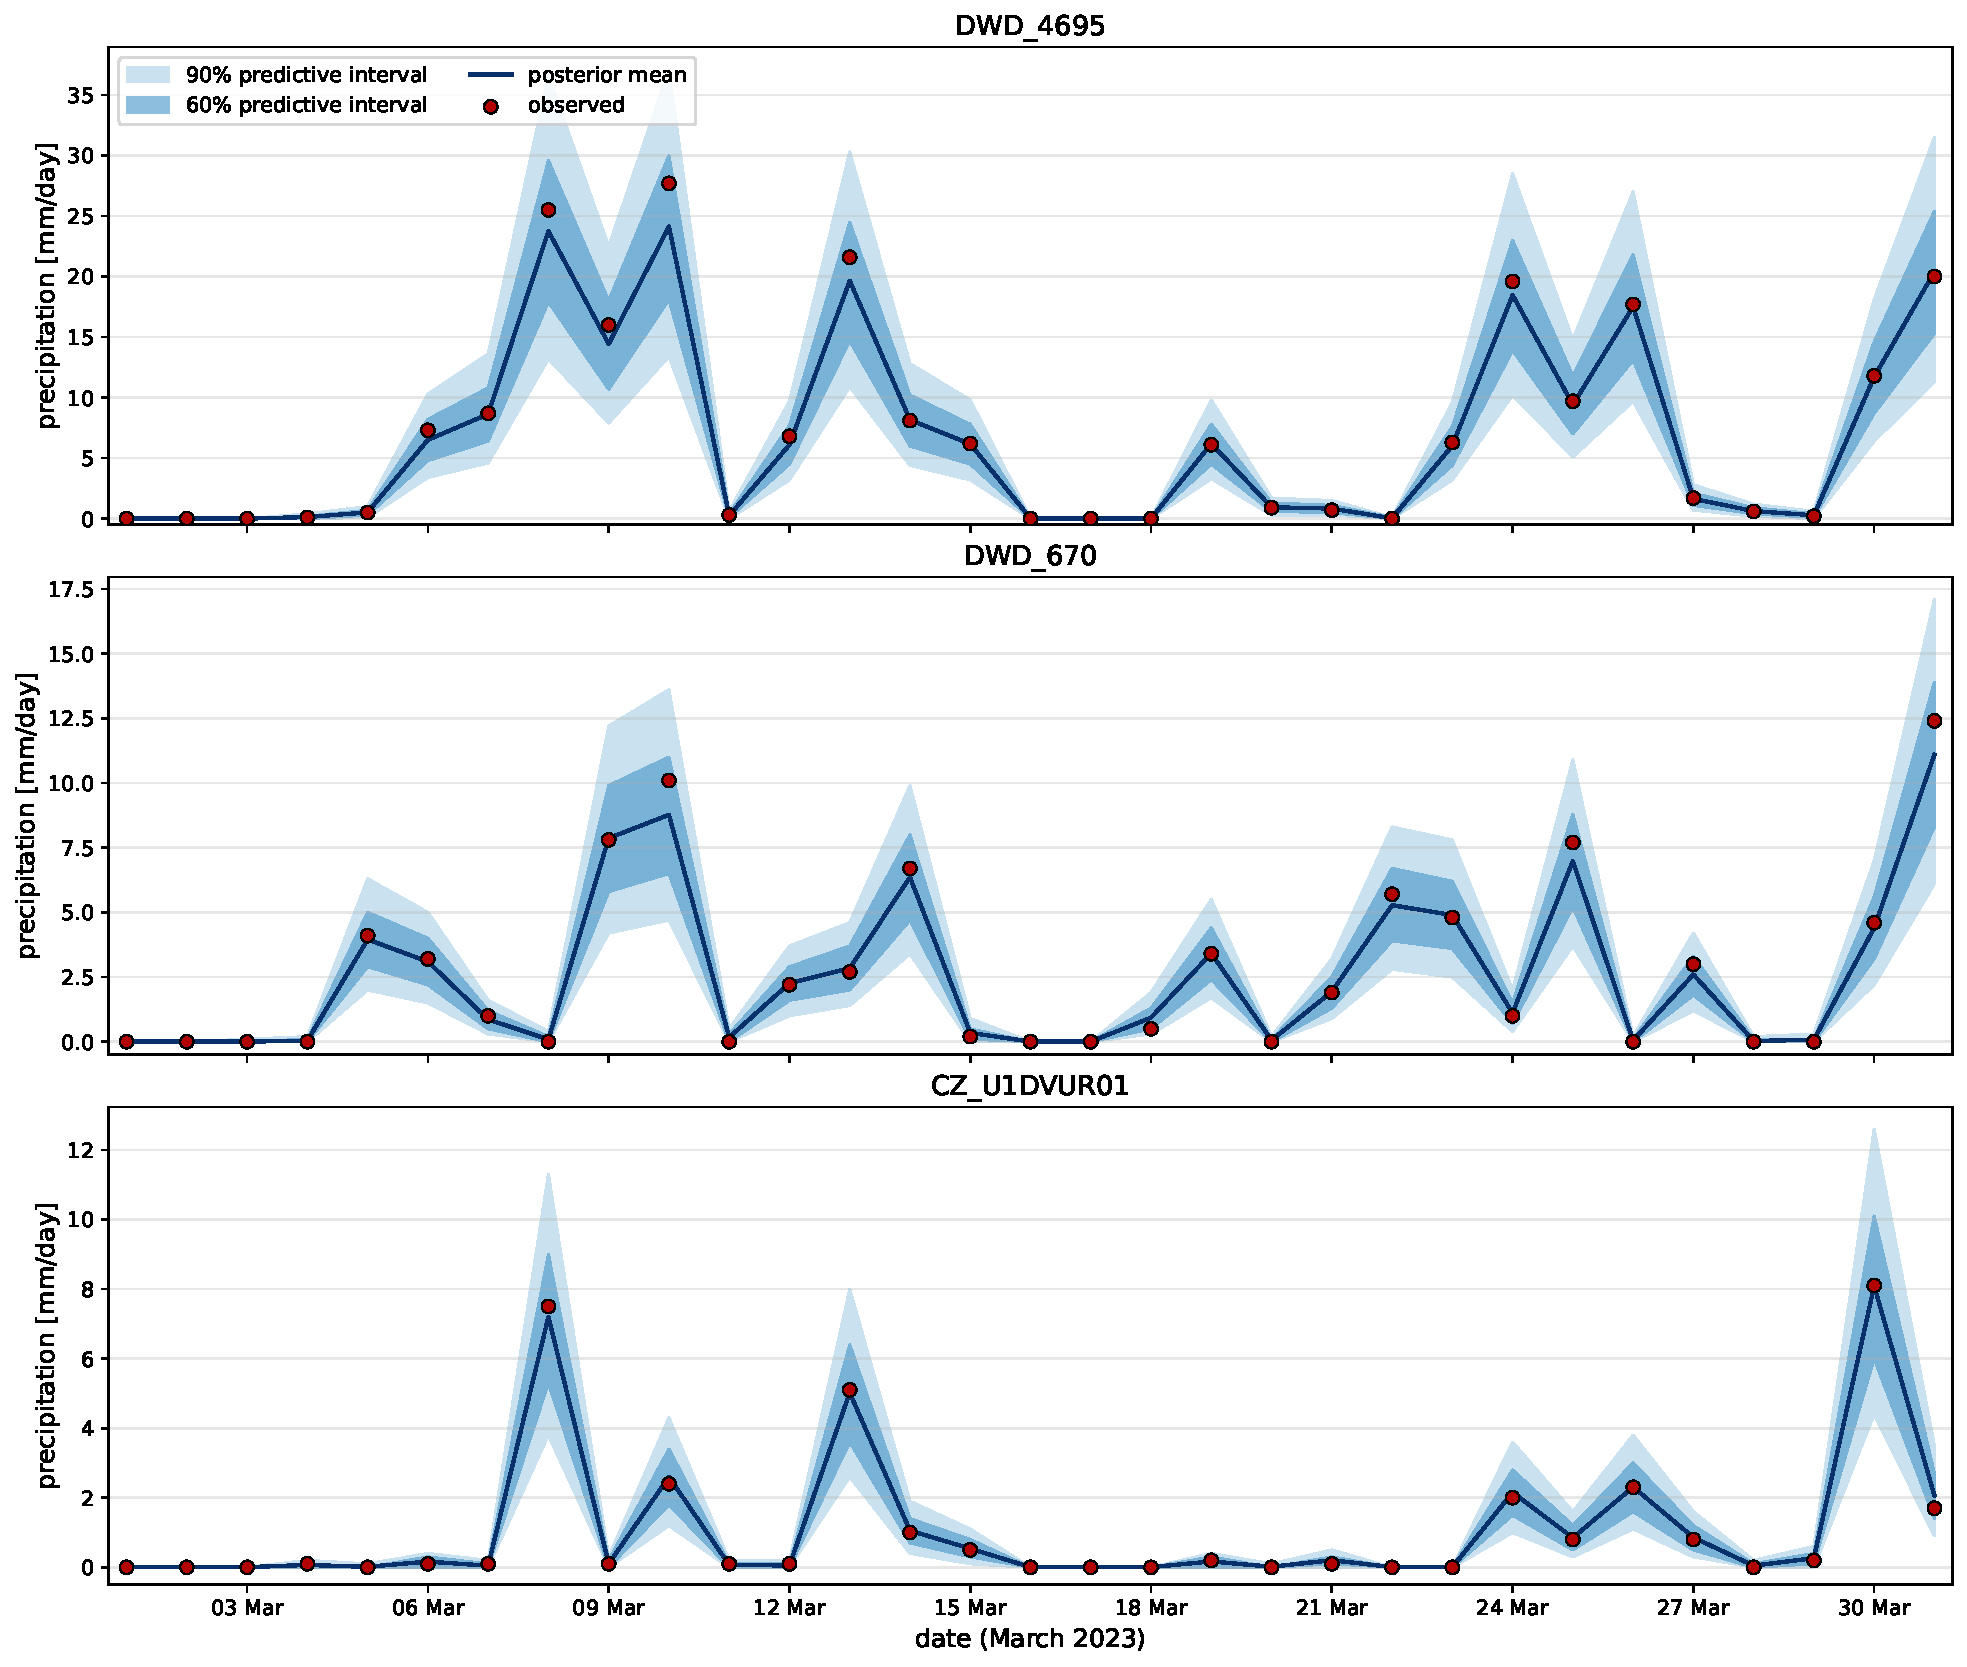
\includegraphics[width=\linewidth]{images/06/bayesnf_station_timeseries.pdf}
  \caption{Posterior mean ($32$ VI replicas), $60$\,\% and $90$\,\%
  predictive intervals, and held-out observations (red dots) over
  March~$2023$ at three holdout stations.}
  \label{fig:bnf-station-timeseries}
\end{figure}
